This section delves into the critical and often misunderstood concepts
of privacy and anonymity in the context of blockchain technology. While
public blockchains are frequently lauded for their transparency, this
very transparency can pose significant challenges to user privacy. We
will begin by dissecting the nuanced distinctions between anonymity,
pseudonymity, and privacy, and we will explore how these concepts apply
to the blockchain.

A common misconception is that blockchains are inherently anonymous. In
reality, most public blockchains are pseudonymous, meaning that users
are identified by cryptographic addresses rather than their real-world
identities. However, as we will see, this pseudonymity can be
compromised through various de-anonymization techniques. We will examine
several of these techniques, including address clustering and
network-level analysis, to understand how the privacy of blockchain
users can be undermined.
%
In response to these privacy challenges, a range of privacy-enhancing
technologies has been developed. We will explore several of these
technologies in detail, including:

\begin{itemize}
\tightlist
\item
  \textbf{Mixing services}, which aim to obscure the link between the
  sender and receiver of a transaction.
\item
  \textbf{Ring signatures}, a cryptographic technique that allows a user
  to sign a transaction on behalf of a group without revealing their
  individual identity.
\item
  \textbf{Zero-knowledge proofs}, a powerful cryptographic tool that
  enables a user to prove the validity of a statement without revealing
  any information beyond the statement's truthfulness.
\end{itemize}

By the end of this section, you will have understanding
of the privacy landscape of blockchain technology, from the inherent
challenges of public ledgers to the cutting-edge cryptographic
techniques that are being used to build a more private and anonymous
future.

\subsection{Learning Objectives}\label{learning-objectives}

\begin{itemize}
\tightlist
\item
  Understand the difference between anonymity, pseudonymity, and
  privacy.
\item
  Learn about the techniques used to de-anonymize blockchain users, such
  as address clustering and network-level analysis.
\item
  Grasp the concept of mixing services and how they can be used to
  enhance privacy.
\item
  Understand the principles of ring signatures and their application in
  privacy-focused cryptocurrencies like Monero~\cite{moser2017empirical}.
\item
  Learn about zero-knowledge proofs and their role in enabling private
  transactions.
\item
  Gain insight into the workings of privacy-focused protocols like
  Zerocoin~\cite{miers2013zerocoin} and Zerocash~\cite{sasson2014zerocash}, and their implementation in Zcash~\cite{kappos2018empirical}.
\end{itemize}

\begin{center}\rule{0.5\linewidth}{0.5pt}\end{center}

\subsection{The Landscape of Anonymity and
Privacy}\label{section-1-the-landscape-of-anonymity-and-privacy}

\subsubsection{Defining Anonymity, Privacy, and
Unlinkability}\label{defining-anonymity-privacy-and-unlinkability}

In the context of blockchain technology, the terms anonymity and privacy
are often used interchangeably, but they refer to distinct, albeit
related, concepts.
%
%\begin{figure}
%\centering
%%\pandocbounded{\includegraphics[keepaspectratio,alt={Anonymity vs Privacy}]{../Input/BDA-07-Anonymity-and-privacy-28.-3.-2024_files/slide_3.png}}
%\caption{Anonymity vs Privacy}
%\end{figure}

\begin{itemize}
\item
  \textbf{Anonymity} refers to the state of being unidentifiable. It
  ensures that a user may use a resource or service without disclosing
  their identity. In a truly anonymous system, it is impossible to link
  actions or transactions to a specific individual. As the transcription
  notes, this is about ``hiding identity.'' For example, a post on a
  forum may be attributed to a pseudonym, not a real-world identity.
\item
  \textbf{Privacy} is the ability of individuals or groups to determine
  for themselves when, how, and to what extent information about them is
  communicated to others. In the context of blockchains, this refers to
  the ability to conceal the details of a transaction, such as the
  identities of the sender and receiver, and the amount being
  transferred. It's about ``hiding confidential information/actions.''
\item
  \textbf{Unlinkability} is a key property that contributes to both
  anonymity and privacy. It is the inability of an adversary to link
  different actions or transactions to the same user. Achieving
  unlinkability is a major challenge in blockchain design. Specific
  requirements for unlinkability include making it difficult to:

  \begin{itemize}
  \tightlist
  \item
    Link different addresses of the same user.
  \item
    Link different transactions made by the same user.
  \item
    Link the sender of a payment to its recipient.
  \end{itemize}
\end{itemize}

Most public blockchains, like Bitcoin, do not provide true anonymity.
Instead, they offer \textbf{pseudonymity}, where users are identified by
cryptographic addresses. The combination of pseudonymity and
unlinkability is what constitutes anonymity on a blockchain.

%\begin{figure}
%\centering
%%\pandocbounded{\includegraphics[keepaspectratio,alt={Anonymity, Pseudonymity, Unlinkability}]{../Input/BDA-07-Anonymity-and-privacy-28.-3.-2024_files/slide_4.png}}
%\caption{Anonymity, Pseudonymity, Unlinkability}
%\end{figure}

\subsubsection{The Anonymity Set}\label{the-anonymity-set}

The \textbf{Anonymity Set} is a crucial concept in this domain. It
refers to the set of transactions that an adversary cannot distinguish
from a specific transaction. The larger the anonymity set, the
greater the privacy, as it becomes harder to single out any individual
transaction. This concept is particularly important when we discuss
techniques like mixing and ring signatures.

%\begin{figure}
%\centering
%%\pandocbounded{\includegraphics[keepaspectratio,alt={Unlinkability \& Anonymity Set}]{../Input/BDA-07-Anonymity-and-privacy-28.-3.-2024_files/slide_5.png}}
%\caption{Unlinkability \& Anonymity Set}
%\end{figure}

\begin{center}\rule{0.5\linewidth}{0.5pt}\end{center}

\subsection{De-anonymization
Techniques}\label{section-2-de-anonymization-techniques}

The pseudonymity of public blockchains can be compromised through a
variety of de-anonymization techniques, which aim to link blockchain
addresses to real-world identities.

%\begin{figure}
%\centering
%%\pandocbounded{\includegraphics[keepaspectratio,alt={De-anonymization}]{../Input/BDA-07-Anonymity-and-privacy-28.-3.-2024_files/slide_6.png}}
%\caption{De-anonymization}
%\end{figure}

\subsubsection{Address Clustering and
Linking}\label{address-clustering-and-linking}

This technique involves analyzing the transaction graph to identify
addresses that are likely controlled by the same entity.



\begin{figure}[t]
	%	\vspace{-0.3cm}
	\begin{center}
		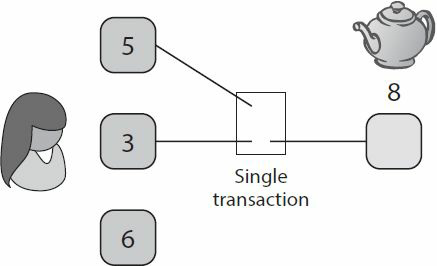
\includegraphics[width=0.4\textwidth]{./figs/deanon1.png}
		\caption{Multiple input addresses controlled by the same user.}		
		\label{fig:deanon1}
	\end{center}	
\end{figure}

\begin{itemize}
\tightlist
\item
  \textbf{Common-input-ownership heuristic}: If multiple addresses (and
  their corresponding UTXOs) are used as inputs in a single transaction,
  it is highly probable that they belong to the same user (see \autoref{fig:deanon1}).
\item
  \textbf{Change Addresses}: When a user sends a transaction and the
  input amount is greater than the output, the remaining ``change'' is
  sent back to a new address. This change address is controlled by the
  same user, creating a link between the input addresses and the new
  change address (see \autoref{fig:deanon2}).
\end{itemize}

\begin{figure}[t]
	%	\vspace{-0.3cm}
	\begin{center}
		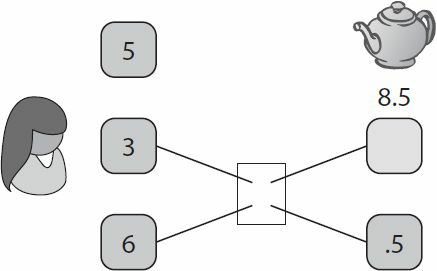
\includegraphics[width=0.4\textwidth]{./figs/deanon2.png}
		\caption{The change address controlled by the same user.}		
		\label{fig:deanon2}
	\end{center}	
\end{figure}

%\begin{figure}
%\centering
%%\pandocbounded{\includegraphics[keepaspectratio,alt={Linking Addresses Example}]{../Input/BDA-07-Anonymity-and-privacy-28.-3.-2024_files/slide_7.png}}
%\caption{Linking Addresses Example}
%\end{figure}

Once a cluster of addresses has been identified, it can be linked to a
real-world identity through various means:

\begin{itemize}
\tightlist
\item
  \textbf{Transacting with Service Providers}: Centralized services like
  cryptocurrency exchanges often require Know Your Customer (KYC)
  verification, linking a user's identity to their deposit and
  withdrawal addresses.
\item
  \textbf{Publicly Advertised Addresses}: Users may post their addresses
  online for donations or payments, directly linking the address to
  their online persona or real identity.
\item
  \textbf{Carelessness}: Users might inadvertently reveal connections
  between their addresses through their online activities.
\end{itemize}

%\pandocbounded{\includegraphics[keepaspectratio,alt={Clustering and Linking to Identities}]{../Input/BDA-07-Anonymity-and-privacy-28.-3.-2024_files/slide_8.png}}
%\pandocbounded{\includegraphics[keepaspectratio,alt={Linking to Individuals}]{../Input/BDA-07-Anonymity-and-privacy-28.-3.-2024_files/slide_9.png}}

\subsubsection{Network-level
De-anonymization}\label{network-level-de-anonymization}

A more sophisticated de-anonymization technique involves monitoring
network traffic to link IP addresses to blockchain transactions. An
adversary with control over a significant portion of the network, such
as an Internet Service Provider (ISP), could potentially use this
technique. When a new transaction is broadcast, it often originates from
a non-full node (like an SPV or light client). The first IP address to
broadcast this transaction is likely the originator.

The solution to this is to use network-layer anonymization tools like
Tor, JonDonym, or VPNs to obscure the user's real IP address.

%\begin{figure}
%\centering
%%\pandocbounded{\includegraphics[keepaspectratio,alt={Network-level De-anonymization}]{../Input/BDA-07-Anonymity-and-privacy-28.-3.-2024_files/slide_10.png}}
%\caption{Network-level De-anonymization}
%\end{figure}

\begin{center}\rule{0.5\linewidth}{0.5pt}\end{center}

\subsection{Privacy-Enhancing
Technologies}\label{section-3-privacy-enhancing-technologies}

\subsubsection{Mixing Services
(Tumblers)}\label{mixing-services-tumblers}

Mixing services are designed to obscure the link between the sender and
receiver of a transaction by mixing a user's coins with those of other
users.

%\begin{figure}
%\centering
%%\pandocbounded{\includegraphics[keepaspectratio,alt={Mixing Services}]{../Input/BDA-07-Anonymity-and-privacy-28.-3.-2024_files/slide_11.png}}
%\caption{Mixing Services}
%\end{figure}

\begin{itemize}
\tightlist
\item
  \textbf{Centralized Mixers}: These services operate as trusted
  intermediaries. A user sends coins to the mixer, which puts them into
  a large pool with coins from other users. The mixer then sends out the
  equivalent amount from this pool to the intended recipient, breaking
  the on-chain link. This approach requires users to trust the mixer not
  to steal their funds or to keep logs of their transactions.
\end{itemize}

%\begin{figure}
%\centering
%%\pandocbounded{\includegraphics[keepaspectratio,alt={Centralized Mixing}]{../Input/BDA-07-Anonymity-and-privacy-28.-3.-2024_files/slide_12.png}}
%\caption{Centralized Mixing}
%\end{figure}

\begin{itemize}
\tightlist
\item
  \textbf{Decentralized Mixers (e.g., CoinJoin)}: To address the trust issue
  of centralized mixers, decentralized mixing protocols like CoinJoin
  have been developed. CoinJoin is a peer-to-peer protocol that allows
  multiple users to collaboratively create a single transaction that
  combines their inputs and outputs (see \autoref{fig:coinjoin}). This makes it difficult for an
  external observer to determine the exact mapping between the inputs
  and outputs, thereby enhancing the privacy of the participants. The
  process involves finding peers, exchanging input/output addresses
  anonymously, constructing a joint transaction, and having all
  participants sign it.
\end{itemize}

\begin{figure}[t]
	%	\vspace{-0.3cm}
	\begin{center}
		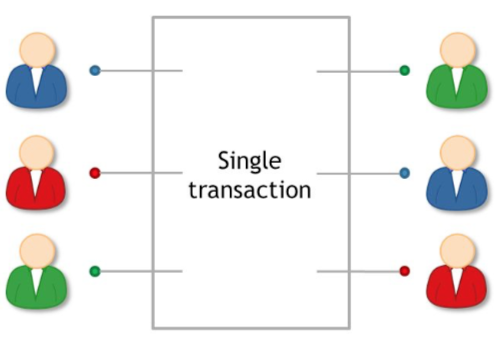
\includegraphics[width=0.4\textwidth]{./figs/coinjoin.png}
		\caption{A single transaction of CoinJoin.}		
		\label{fig:coinjoin}
	\end{center}	
\end{figure}

%\pandocbounded{\includegraphics[keepaspectratio,alt={CoinJoin}]{../Input/BDA-07-Anonymity-and-privacy-28.-3.-2024_files/slide_13.png}}
%\pandocbounded{\includegraphics[keepaspectratio,alt={CoinJoin Process}]{../Input/BDA-07-Anonymity-and-privacy-28.-3.-2024_files/slide_14.png}}

\subsubsection{Ring Signatures}\label{ring-signatures}

A ring signature is a cryptographic technique that allows a member of a
group to sign a message on behalf of the group, without revealing which
member of the group produced the signature. This provides a high degree
of sender anonymity.

%\begin{figure}
%\centering
%%\pandocbounded{\includegraphics[keepaspectratio,alt={Ring Signatures}]{../Input/BDA-07-Anonymity-and-privacy-28.-3.-2024_files/slide_15.png}}
%\caption{Ring Signatures}
%\end{figure}

The key properties are: (A) The actual signer declares an arbitrary set of
possible signers (the ``ring''), which includes themselves. (B) The
signature is constructed using the signer's private key and the public
keys of all other ring members. (C) No interaction is required between the
ring members. (D) An adversary cannot distinguish which member of the ring
is the true signer.

%\begin{figure}
%\centering
%%\pandocbounded{\includegraphics[keepaspectratio,alt={Ring Signature Properties}]{../Input/BDA-07-Anonymity-and-privacy-28.-3.-2024_files/slide_17.png}}
%\caption{Ring Signature Properties}
%\end{figure}

\paragraph{Generating and Verifying a Ring
Signature.}\label{generating-and-verifying-a-ring-signature}

The process, illustrated with an RSA example, involves several steps: 
\begin{enumerate}
	\item The signer hashes the message \texttt{m} to create a symmetric key
	\texttt{k}.
	
	\item A random value \texttt{v} is generated by signer. 
	
	\item  For all other ring members, signer generates random values \texttt{$x_i$} and corresponding
	$y_i = g_i(x_i)$ values are computed using a \textbf{trapdoor} function (e.g.,
	$y_i\ =\ x_i^{e_i}\ mod\ n_i$ in RSA). 
	
	\item  Given a symmetric encryption algorithm $E_k$, we define a combining function
	$C_{k,v}$ that is used to create a loop, and the signer solves for their
	own $y_s$ value by fitting the equation 
	($C_{k,v}(...)\ =\ v$).  
	See also \autoref{fig:ring} and \autoref{fig:ring2}. 
	
	\item The signer computes their private key  $x_s = g_{s^{-1}}(y_s)$ using the knowledge of trapdoor from $y_s$. 
	E.g. in RSA: $x_s = y_{s}^{d_s}\ mod\ n_s$ 
	 
	 \item  The final signature consists of the public keys of all ring members, the value \texttt{v}, and all the \texttt{x} values, i.e., ($P_1, P_2, \ldots, P_r, v, x_1, x_2, \ldots, x_s, \ldots, x_r$). 
	
\end{enumerate}


\begin{figure}[t]
	%	\vspace{-0.3cm}
	\begin{center}
		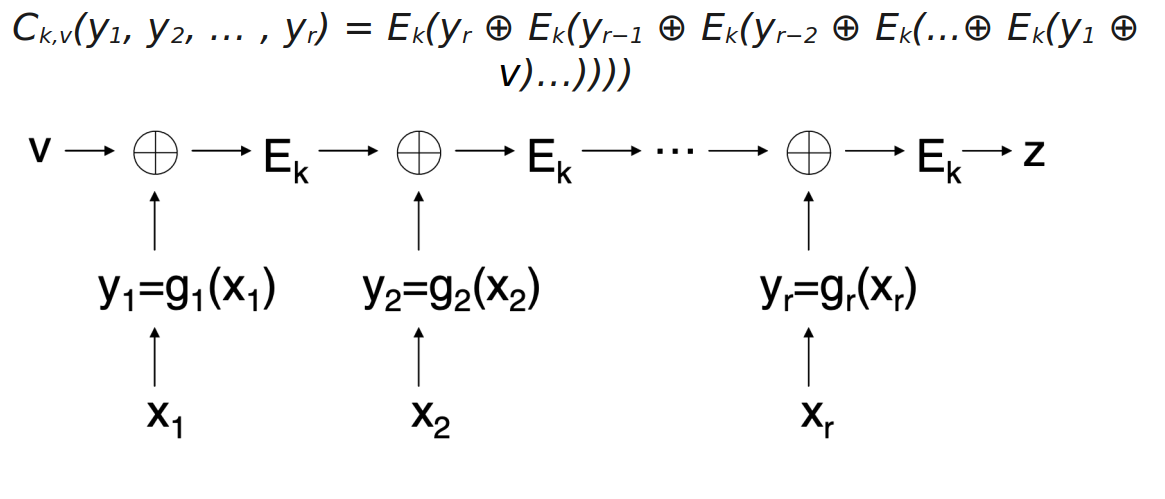
\includegraphics[width=0.7\textwidth]{./figs/ring-sig.png}
		\caption{Combining function in a ring signature.}		
		\label{fig:ring}
	\end{center}	
\end{figure}


\begin{figure}
	%	\vspace{-0.3cm}
	\begin{center}
		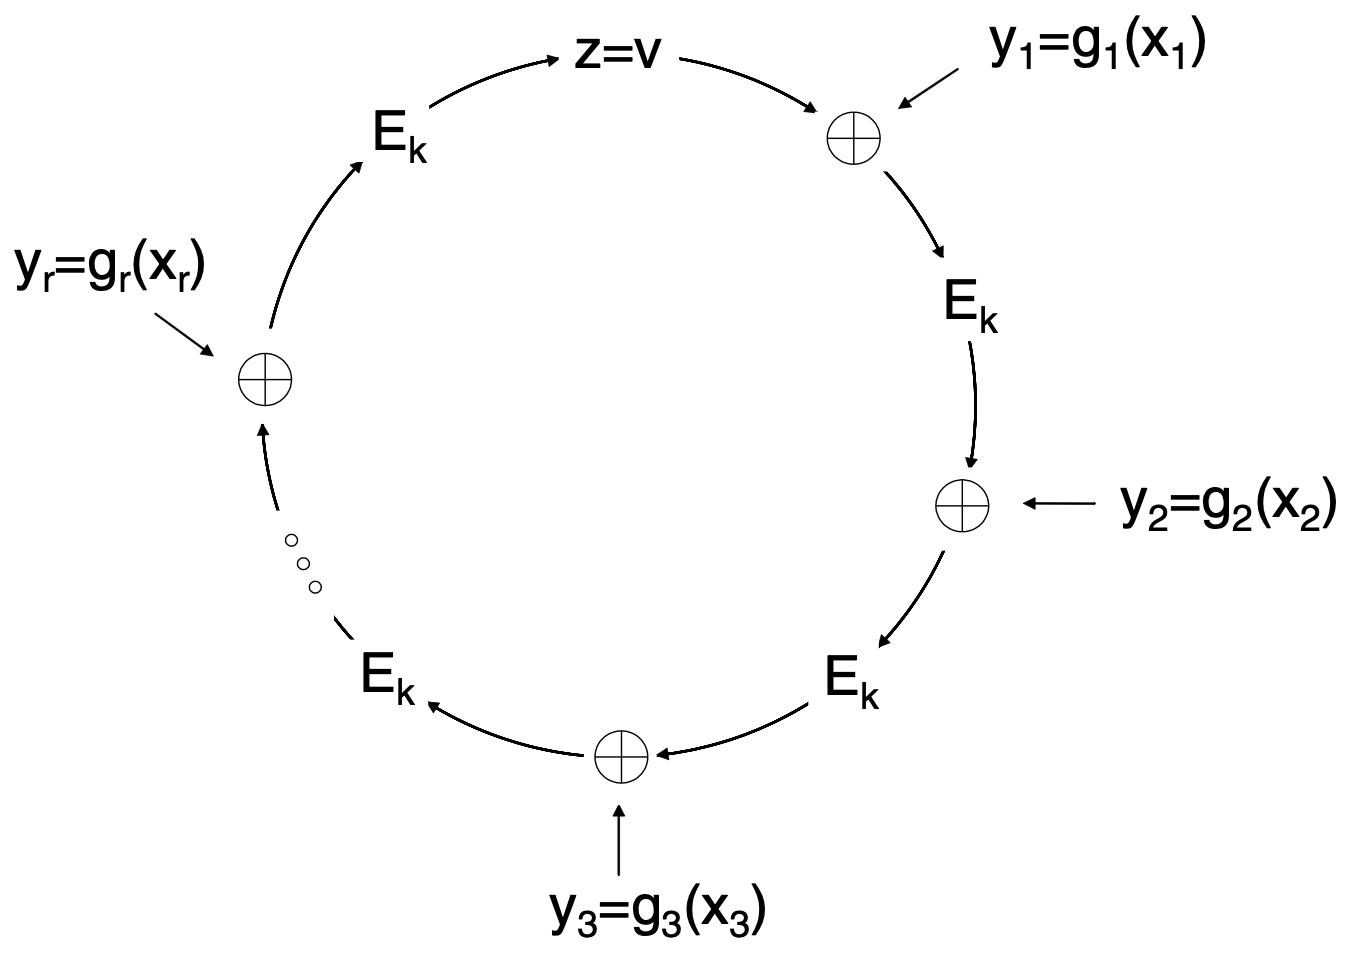
\includegraphics[width=0.5\textwidth]{./figs/ring2.png}
		\caption{Combining function equal to $v$ in a ring signature.}		
		\label{fig:ring2}
	\end{center}	
\end{figure}

Verification involves checking that the equation holds true using the
public keys and the provided signature components.
In particular, given a message \textbf{m} and alleged signature ($P_1, P_2, \ldots, P_r, v, x_1, x_2, \ldots, x_s, \ldots, x_r$), the signature is verified as follows:

\begin{enumerate}
	\item For $i = 1,2,3, \ldots, r$, the verifier computes $y_i = g_i (x_i)$.
	
	\item The verifier hashes the message to obtain the symmetric encryption key $k = H(m)$.
	
	\item The verifier checks that the $y_i$’s computed in 1) satisfy the equation $C_{k,v}(y_1, y_2, …, y_r) = v$
	
\end{enumerate}
	


%\pandocbounded{\includegraphics[keepaspectratio,alt={Generating a Ring Signature 1}]{../Input/BDA-07-Anonymity-and-privacy-28.-3.-2024_files/slide_18.png}}
%\pandocbounded{\includegraphics[keepaspectratio,alt={Generating a Ring Signature 2}]{../Input/BDA-07-Anonymity-and-privacy-28.-3.-2024_files/slide_19.png}}
%\pandocbounded{\includegraphics[keepaspectratio,alt={Generating a Ring Signature 3}]{../Input/BDA-07-Anonymity-and-privacy-28.-3.-2024_files/slide_20.png}}
%\pandocbounded{\includegraphics[keepaspectratio,alt={Verifying a Ring Signature}]{../Input/BDA-07-Anonymity-and-privacy-28.-3.-2024_files/slide_21.png}}

\paragraph{Monero.}\label{monero}
The privacy-focused cryptocurrency Monero is the most well-known
application of ring signatures. 
It uses two key pairs: \textbf{viewing
keys} and \textbf{spending keys}. \textbf{Stealth addresses} are used
for recipient anonymity; a new one-time address is generated for each
transaction. \textbf{Key images} are used to prevent double-spending.
A unique key image is derived from each output, and the blockchain
maintains a list of spent key images. \textbf{RingCT (Ring
Confidential Transactions)} hides transaction amounts using Pedersen
commitments and zero-knowledge range proofs.



%\pandocbounded{\includegraphics[keepaspectratio,alt={Monero}]{../Input/BDA-07-Anonymity-and-privacy-28.-3.-2024_files/slide_22.png}}
%\pandocbounded{\includegraphics[keepaspectratio,alt={Monero Details}]{../Input/BDA-07-Anonymity-and-privacy-28.-3.-2024_files/slide_23.png}}
%\pandocbounded{\includegraphics[keepaspectratio,alt={Monero Key Images \& RingCT}]{../Input/BDA-07-Anonymity-and-privacy-28.-3.-2024_files/slide_24.png}}

\subsubsection{Zero-Knowledge Proofs}\label{zero-knowledge-proofs}

A zero-knowledge proof (ZKP) is a powerful cryptographic protocol that
allows one party (the prover) to prove to another party (the verifier)
that a statement is true, without revealing any information beyond the
validity of the statement itself.

%\begin{figure}
%\centering
%%\pandocbounded{\includegraphics[keepaspectratio,alt={Zero-Knowledge Proofs}]{../Input/BDA-07-Anonymity-and-privacy-28.-3.-2024_files/slide_25.png}}
%\caption{Zero-Knowledge Proofs}
%\end{figure}

The classic ``Ali Baba Cave'' example illustrates the concept of an
interactive proof (see \autoref{fig:alibaba}). However, for blockchains, non-interactive proofs are
needed. The \textbf{Fiat-Shamir heuristic} is a technique to convert
interactive proofs into non-interactive ones by replacing the verifier's
challenge with the output of a hash function~\cite{fiat1986prove}.


\begin{figure}[t]
	%	\vspace{-0.3cm}
	\begin{center}
		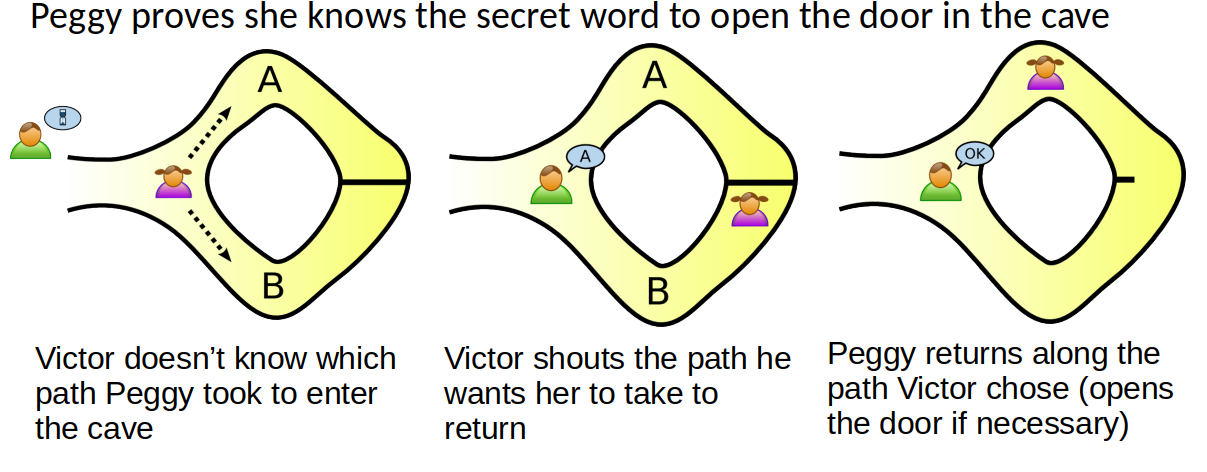
\includegraphics[width=0.8\textwidth]{./figs/alibaba.png}
		\caption{Interactive zero-knowledge proof example of Alibaba cave Verifier has to repeat the query multiple times to decrease a chance of prover to guess it.}		
		\label{fig:alibaba}
	\end{center}	
\end{figure}


%\pandocbounded{\includegraphics[keepaspectratio,alt={Ali Baba Cave}]{../Input/BDA-07-Anonymity-and-privacy-28.-3.-2024_files/slide_26.png}}
%\pandocbounded{\includegraphics[keepaspectratio,alt={Schnorr's Protocol (Interactive)}]{../Input/BDA-07-Anonymity-and-privacy-28.-3.-2024_files/slide_27.png}}
%\pandocbounded{\includegraphics[keepaspectratio,alt={Non-Interactive ZKP}]{../Input/BDA-07-Anonymity-and-privacy-28.-3.-2024_files/slide_28.png}}

\paragraph{zk-SNARKs}\label{zk-snarks}

\textbf{Zero-Knowledge Succinct Non-interactive ARguments of Knowledge
(zk-SNARKs).} are a specific type of ZKP ideal for blockchains because
their proofs are very small (``succinct'') and quick to verify. They
allow a party to prove the correctness of a complex computation without
revealing the inputs and without requiring the verifier to re-run the
entire computation.
%
%\begin{figure}
%\centering
%%\pandocbounded{\includegraphics[keepaspectratio,alt={zk-SNARKs}]{../Input/BDA-07-Anonymity-and-privacy-28.-3.-2024_files/slide_29.png}}
%\caption{zk-SNARKs}
%\end{figure}

\subsubsection{Schnorr's Prtocol -- Discrete Log. Problem}\label{sec:schnorr}
Schnorr's protocol represents interactive proving of knowledge of discrete logarithm.
In particular, prover wants to prove the knowledge of discrete logarithm $x$ of
$h = g^x \in G$, where $G$ is a group of prime order $q$ (see \autoref{fig:schnorr-inter}).

\begin{figure}[h]
	%	\vspace{-0.3cm}
	\begin{center}
		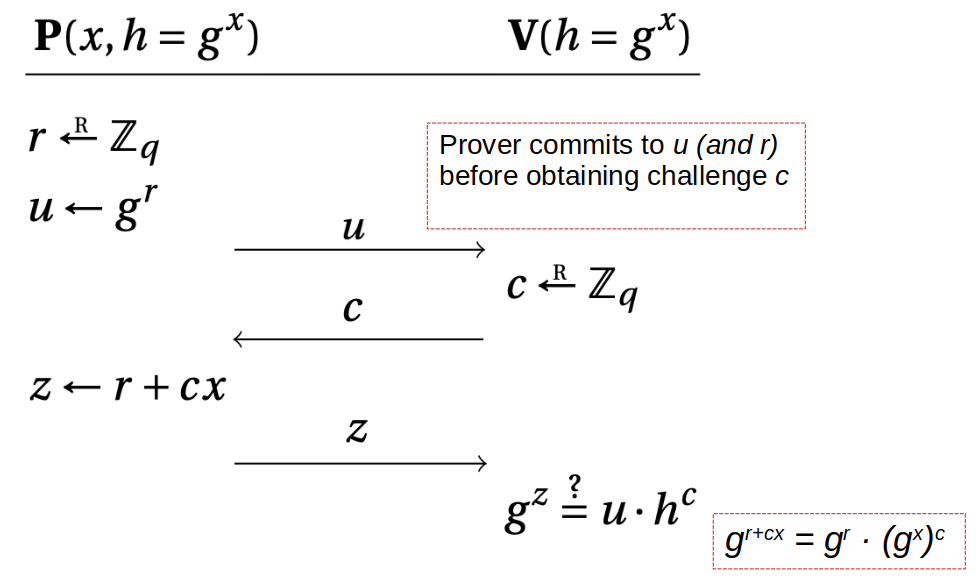
\includegraphics[width=0.4\textwidth]{./figs/schnor-inter.png}
		\caption{Schnorr's interactive protocol.}		
		\label{fig:schnorr-inter}
	\end{center}	
\end{figure}


\medskip
\textbf{Non-Interactive Variant.} 
Using Fiat-Shamir heuristic, we can convert interactive Schnorr's protocol to non-interactive protocol in random oracle model. 
In particular, the challenge $c$ is replaced by the hash cryptographicaly secure hash function (see \autoref{fig:schnorr-noninter}).
\begin{figure}[h]
	%	\vspace{-0.3cm}
	\begin{center}
		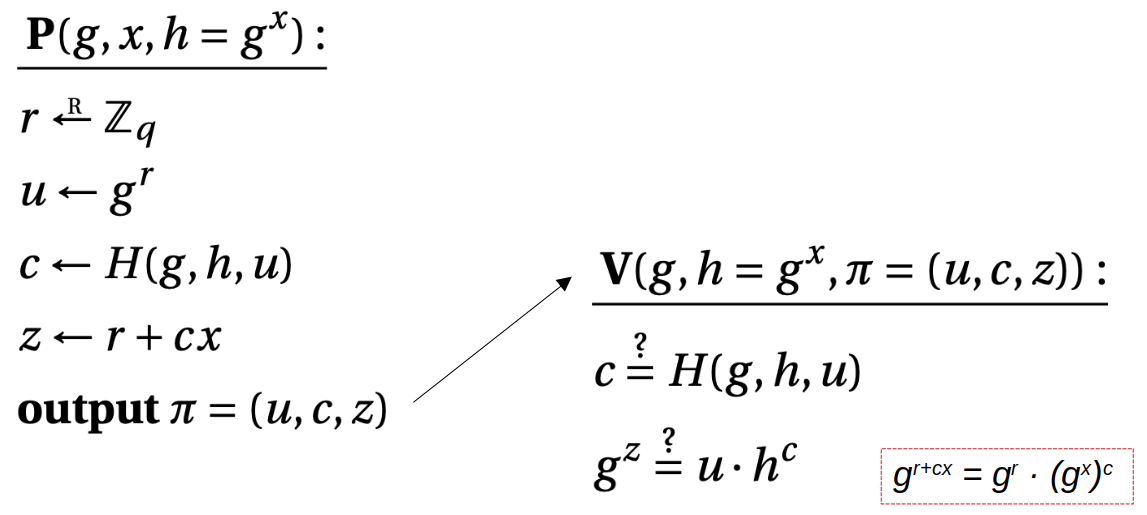
\includegraphics[width=0.5\textwidth]{./figs/schnor-noninter.png}
		\caption{Schnorr's non-interactive protocol.}		
		\label{fig:schnorr-noninter}
	\end{center}	
\end{figure}





\subsubsection{Zcash (Zerocoin and Zerocash
Protocols)}\label{zcash-zerocoin-and-zerocash-protocols}

Zcash is a cryptocurrency that implements these advanced ZKP concepts.

%\begin{figure}
%\centering
%%\pandocbounded{\includegraphics[keepaspectratio,alt={Zcash}]{../Input/BDA-07-Anonymity-and-privacy-28.-3.-2024_files/slide_30.png}}
%\caption{Zcash}
%\end{figure}

\begin{itemize}
\tightlist
\item
  \textbf{Zerocoin Protocol}: The original protocol proposed for
  Bitcoin. It allows a user to ``burn'' a coin and ``mint'' a new,
  anonymous one with no transaction history, using a ZKP to prove
  ownership.
\end{itemize}

%\begin{figure}
%\centering
%%\pandocbounded{\includegraphics[keepaspectratio,alt={Zerocoin Protocol}]{../Input/BDA-07-Anonymity-and-privacy-28.-3.-2024_files/slide_31.png}}
%\caption{Zerocoin Protocol}
%\end{figure}

\begin{itemize}
\tightlist
\item
  \textbf{Zerocash Protocol}: An extension of Zerocoin that uses
  zk-SNARKs to make the proofs much smaller and to hide not only the
  origin but also the destination and amount of the transaction. A
  critical aspect of this protocol is the need for a \textbf{trusted
  setup}, where initial public parameters are generated from random data
  that must then be destroyed to prevent counterfeiting. Modern
  implementations use multi-party computation (MPC) ceremonies to
  distribute this trust.
\end{itemize}

%\begin{figure}
%\centering
%%\pandocbounded{\includegraphics[keepaspectratio,alt={Zerocash Protocol}]{../Input/BDA-07-Anonymity-and-privacy-28.-3.-2024_files/slide_32.png}}
%\caption{Zerocash Protocol}
%\end{figure}

\begin{itemize}
\tightlist
\item
  \textbf{Zcash Implementation}: Zcash uses two types of addresses:

  \begin{itemize}
  \tightlist
  \item
    \textbf{t-addresses} (transparent)
  \item
    \textbf{z-addresses} (private or ``shielded'') These addresses are
    interoperable, allowing for four transaction types: private
    (z-to-z), shielding (t-to-z), deshielding (z-to-t), and public
    (t-to-t).
  \end{itemize}
\end{itemize}

%\begin{figure}
%\centering
%%\pandocbounded{\includegraphics[keepaspectratio,alt={Zcash Blockchain}]{../Input/BDA-07-Anonymity-and-privacy-28.-3.-2024_files/slide_33.png}}
%\caption{Zcash Blockchain}
%\end{figure}

\begin{center}\rule{0.5\linewidth}{0.5pt}\end{center}

\subsection{Summary / Key Takeaways}\label{summary-key-takeaways}

This section has provided an overview of the complex and
often misunderstood topics of privacy and anonymity in the context of
blockchain technology. We have established that while public blockchains
are transparent by design, they are not inherently anonymous, but rather
pseudonymous. This pseudonymity, however, can be compromised through
various de-anonymization techniques.

We have explored several of these techniques, including address
clustering and network-level analysis, which can be used to link
blockchain addresses to real-world identities. In response to these
privacy challenges, a range of privacy-enhancing technologies has been
developed. We have examined several of these technologies in detail,
including:

\begin{itemize}
\tightlist
\item
  \textbf{Mixing services}, which obscure the transaction graph by
  mixing the coins of multiple users.
\item
  \textbf{Ring signatures}, which provide sender anonymity by allowing a
  user to sign a transaction on behalf of a group.
\item
  \textbf{Zero-knowledge proofs}, which enable the verification of
  transactions without revealing any sensitive information.
\end{itemize}

The development of these technologies highlights the ongoing tension
between the transparency and privacy of blockchain systems. As the
technology continues to mature, this will undoubtedly remain a key area
of research and innovation.

\begin{center}\rule{0.5\linewidth}{0.5pt}\end{center}

\subsection{Keywords}\label{keywords}

\begin{itemize}
\tightlist
\item
  \textbf{Anonymity}: The quality or state of being anonymous; the
  condition of having no name or an unknown name.
\item
  \textbf{Privacy}: The state of being free from public attention; the
  ability to control what information is shared with others.
\item
  \textbf{Pseudonymity}: The use of a fictitious name or pseudonym to
  conceal one's true identity.
\item
  \textbf{Unlinkability}: The inability of an adversary to link
  different actions or transactions to the same user.
\item
  \textbf{Mixing Service (Tumbler)}: A service that breaks the link
  between the sender and receiver of a transaction by mixing the coins
  of multiple users.
\item
  \textbf{CoinJoin}: A decentralized mixing protocol that allows
  multiple users to combine their inputs into a single transaction.
\item
  \textbf{Ring Signature}: A type of digital signature that provides
  sender anonymity by allowing a user to sign a transaction on behalf of
  a group of users.
\item
  \textbf{Monero}: A privacy-focused cryptocurrency that uses ring
  signatures, stealth addresses, and RingCT to provide a high degree of
  privacy and anonymity.
\item
  \textbf{Zero-Knowledge Proof (ZKP)}: A cryptographic protocol that
  allows a prover to convince a verifier that a statement is true,
  without revealing any information beyond the validity of the statement
  itself.
\item
  \textbf{zk-SNARKs}: A specific type of zero-knowledge proof that is
  particularly efficient and is used in several privacy-focused
  cryptocurrencies, such as Zcash.
\item
  \textbf{Zcash}: A cryptocurrency that uses zk-SNARKs to provide strong
  privacy guarantees, allowing users to send transactions from shielded
  addresses.
\end{itemize}

\begin{center}\rule{0.5\linewidth}{0.5pt}\end{center}

\subsection{Further Reading}\label{further-reading}

\begin{itemize}
\tightlist
\item
  \textbf{A Fistful of Bitcoins: Characterizing Payments Among Men with
  No Names}: \\
\url{https://cseweb.ucsd.edu/~smeiklejohn/files/imc13.pdf}

\item
  \textbf{How to leak a secret: Theory and applications of ring
  signatures}: \\
  \url{https://link.springer.com/chapter/10.1007/11957454_11}
\item
  \textbf{Traceable ring signature}:\\
  \url{https://link.springer.com/chapter/10.1007/978-3-540-70930-7_12}
\item
  \textbf{Ring confidential transactions}:\\
  \url{https://ledger.pitt.edu/ojs/ledger/article/view/1/1}
\item
  \textbf{Why and how zk-SNARK works}:\\
  \url{https://arxiv.org/pdf/1906.07221.pdf}
\item
  \textbf{Zcash Technology}:\\ \url{https://z.cash/technology/}
\item
  \textbf{Zero-to-Monero}:\\
  \url{https://www.getmonero.org/library/Zero-to-Monero-2-0-0.pdf}
\item
  \textbf{Zerocoin: Anonymous distributed e-cash from bitcoin}:\\
  \url{https://ieeexplore.ieee.org/document/6547123}
\item
  \textbf{Zerocash: Decentralized Anonymous Payments from Bitcoin}:\\
  \url{https://ieeexplore.ieee.org/document/6847623}
\end{itemize}
